So in here we will showcase the different things you can do.

\section{Citation}
\label{sec:citation}
We can cite things from the \emph{bib.tex} file using \verb=\cite{qdraw}= which will change into the appropriate citation style you chose \cite{qdraw}. "qdraw" is the \emph{Citation Key} set for that entry in Mendeley. You can also cite author, \citeauthor{qdraw}, in your text using \verb=\citeauthor{qdraw}=.

We can also cite other chapters, sections, figures, tables if they have a label. For example when we defined this section \verb=\section{Citation}= we added right after it a label \verb=\label{citationSection}= we can reference that section \ref{sec:citation} using \verb=\ref{sec:citation}=, you will notice "\ref{sec:citation}" is inserted and its also a hyperlink to the section.

\section{Labels}
Its best practice to start the labels with the type of objects:
\begin{itemize}
    \item \verb=\label{sec:FollowedWithSectionName}=
    \item \verb=\label{tab:FollowedWithTableName}=
    \item \verb=\label{fig:FollowedWithFigureName}=
    \item \verb=\label{lis:FollowedWithListingName}=
    \item \verb=\label{ch:FollowedWithChapterName}=
\end{itemize}

\section{Adding a SVG}
Using this template you can add an svg figure from your \emph{fig} folder. Inkscape needs to be installed, in the background Inkscape will be run to convert your SVG to a PDF, it will get placed in a folder in the root folder called \emph{svg-inkscape} and used.

\begin{Verbatim}[fontsize=\relsize{-1.5}]
    \begin{figure}[h]
        \centering
        \includesvg[width = 0.25\textwidth]{Firefox}
        \caption{This is a SVG logo.}
        \label{fig:svglogo}
    \end{figure}
\end{Verbatim}

\begin{figure}[h]
    \centering
    \includesvg[width = 0.25\textwidth]{Firefox}
    \caption{This is a SVG logo.}
    \label{fig:svglogo}
\end{figure}
%\pagebreak
\section{Adding an Image}
Its very similar to the SVG. Since in the \emph{Main.tex} file we already set our Graphics Path \verb=\graphicspath{{fig/}}=, we can write directly the name of an image or a folder inside that.
\begin{Verbatim}[fontsize=\relsize{-1.5}]
    \begin{figure}[h]
        \centering
        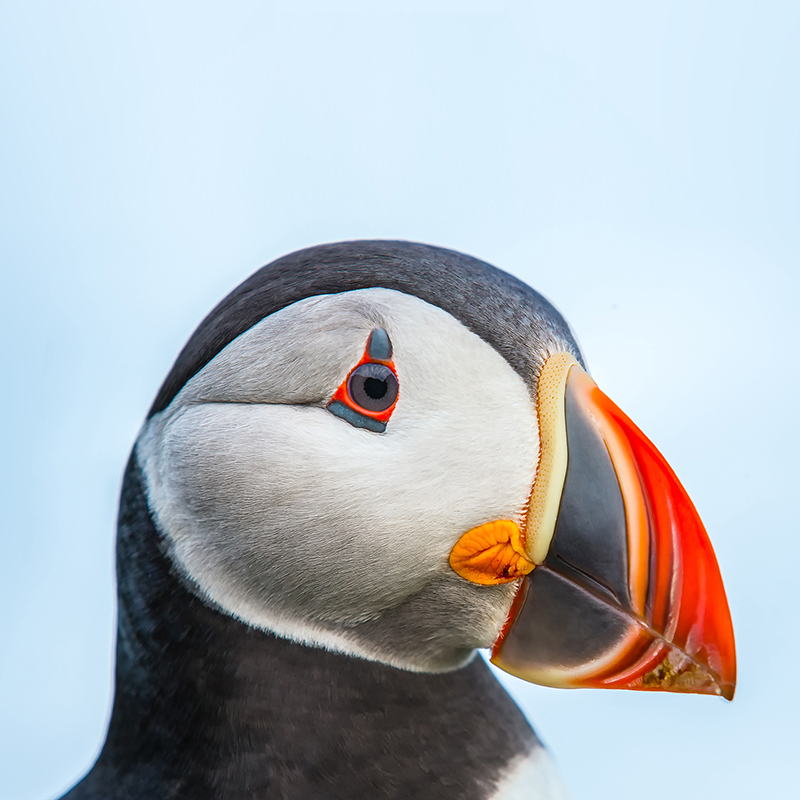
\includegraphics[width=\textwidth]{puffin}
        \caption{This is a puffin...}
        \label{fig:puffin}
    \end{figure}
\end{Verbatim}
\begin{figure}[h]
    \centering
    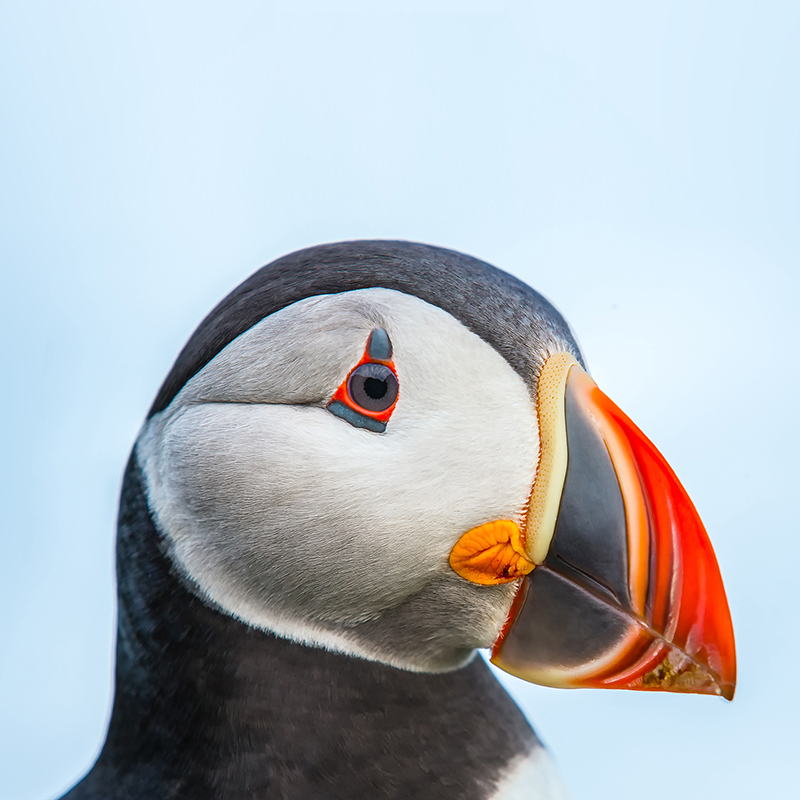
\includegraphics[width=\textwidth]{puffin}
    \caption{This is a puffin...}
    \label{fig:puffin}
\end{figure}

\faWarning\, If you go back to List of Figures, you will notice the two figures we just created were added automatically.

\faWarning\, If you noticed with the SVG and the image we used \verb_width=\textwidth_ using text width allows us to  easily stretch the image to the same width of our text.

\faWarning\, Use \verb=\ref{fig:puffin}= and \verb=\ref{fig:svglogo}= to refer to figure \ref{fig:puffin} and figure \ref{fig:svglogo}.
\pagebreak
\subsection{Multiple images}
You can insert images in a grid. For this we are using the \emph{Subcaption} package. The idea is to use a \emph{subfigure} with a width less than $linewidth$. Check here \url{http://mirrors.ibiblio.org/CTAN/macros/latex/contrib/caption/subcaption.pdf} and here \url{https://tex.stackexchange.com/a/119985} for details.
\begin{Verbatim}[fontsize=\relsize{-1.5}]
    \begin{figure} [H]
        \centering
        \begin{subfigure}[b]{.45\linewidth}
            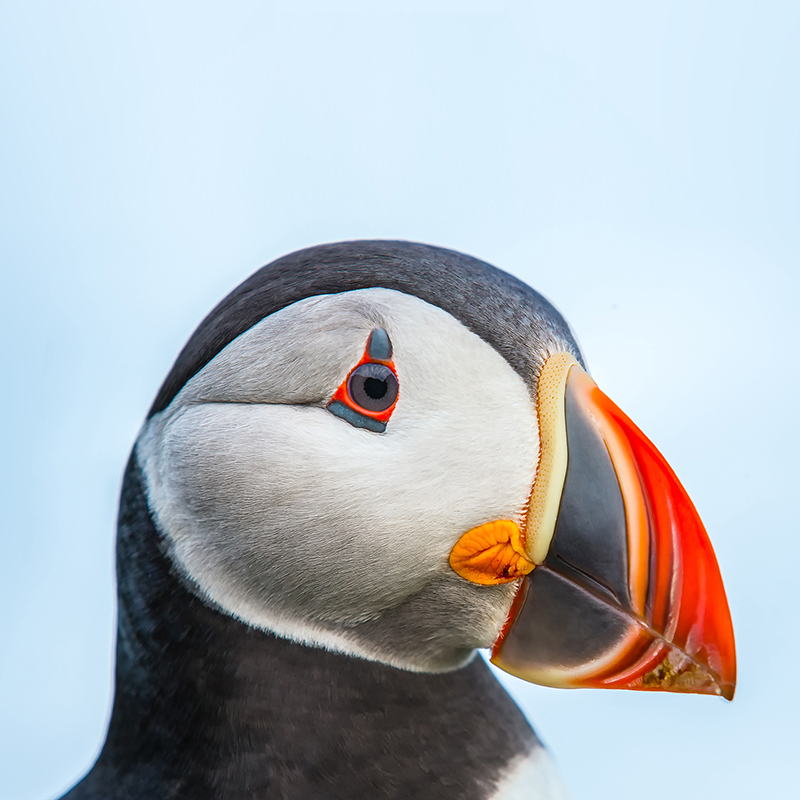
\includegraphics[width=\linewidth]{puffin}
            \caption{Useless Image}\label{fig:puffin1}
        \end{subfigure}
        \begin{subfigure}[b]{.45\linewidth}
            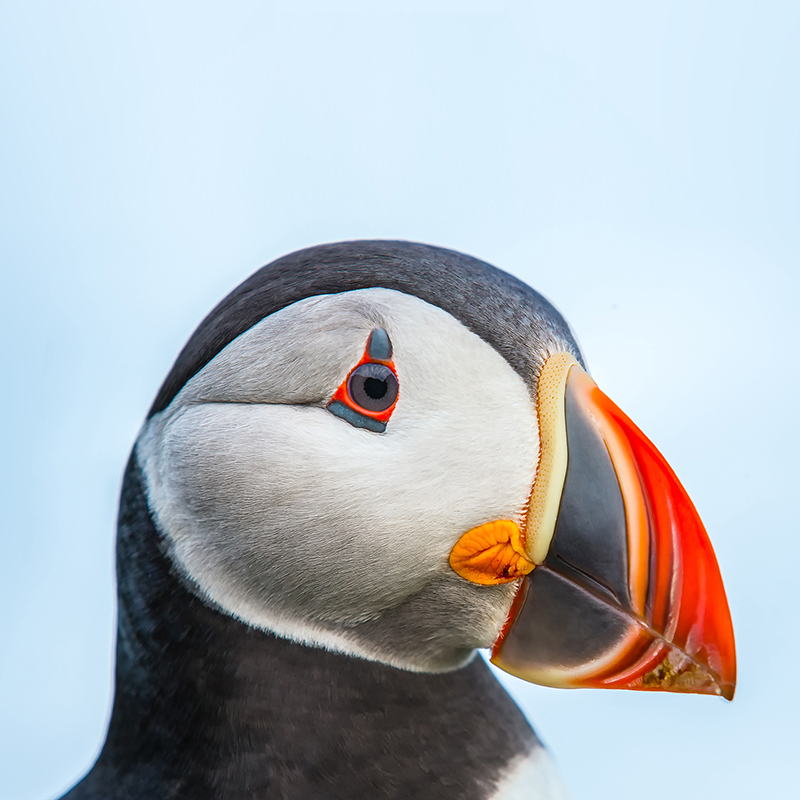
\includegraphics[width=\linewidth]{puffin}
            \caption{puffin Image}\label{fig:puffin2}
        \end{subfigure}

        \begin{subfigure}[b]{.45\linewidth}
            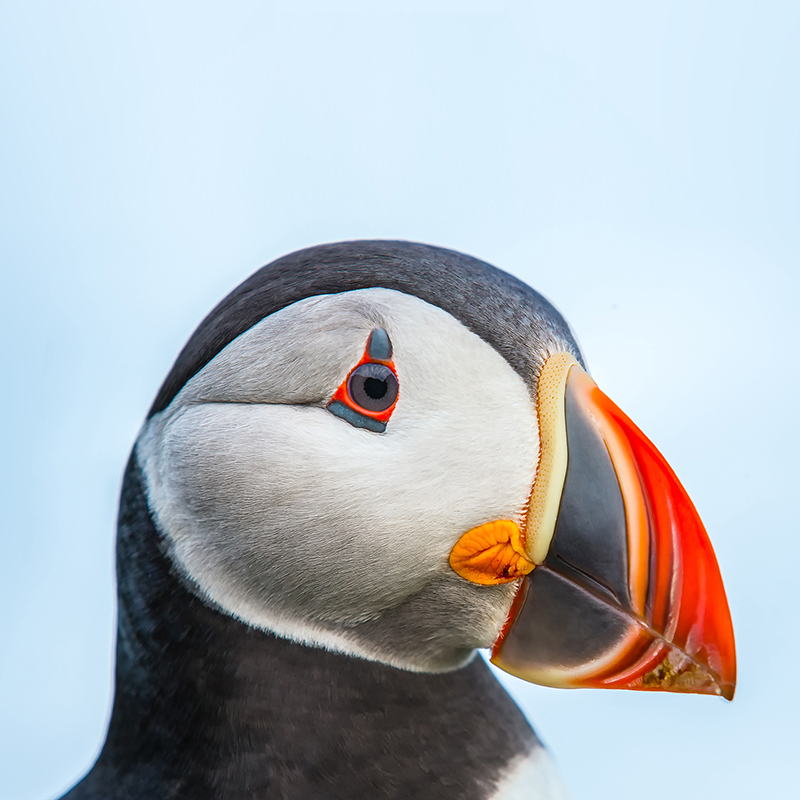
\includegraphics[width=\linewidth]{puffin}
            \caption{puffin Image}\label{fig:puffin4}
        \end{subfigure}
        \begin{subfigure}[b]{.45\linewidth}
            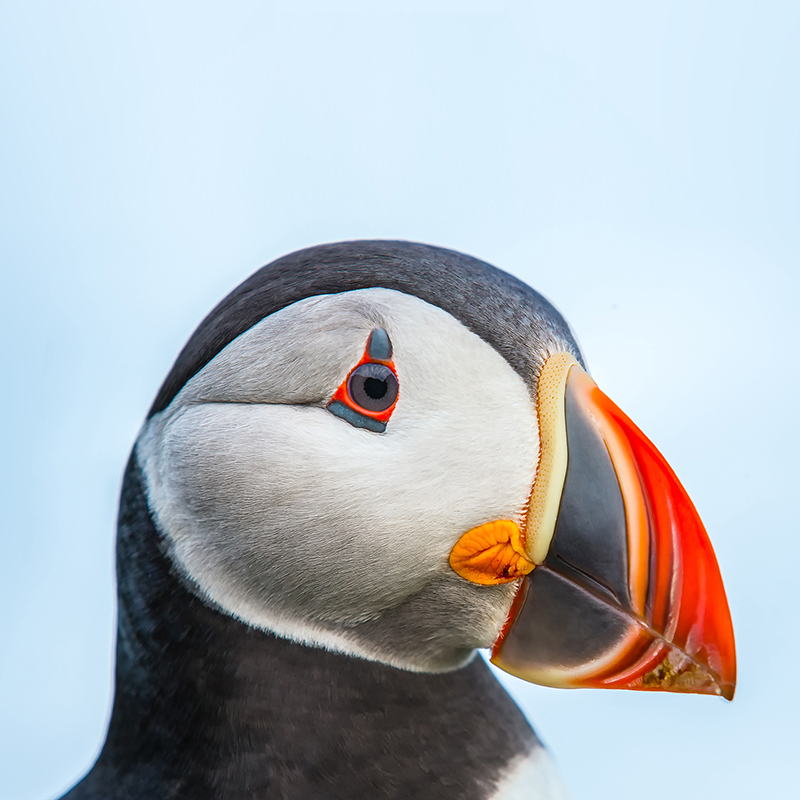
\includegraphics[width=\linewidth]{puffin}
            \caption{puffin Image}\label{fig:puffin5}
        \end{subfigure}

        \begin{subfigure}[b]{.45\linewidth}
            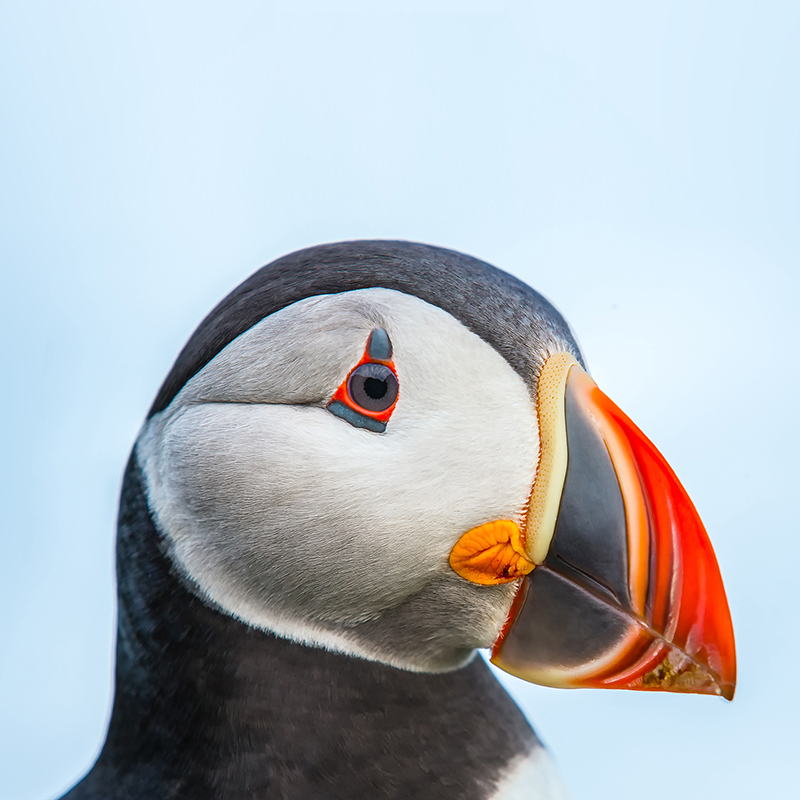
\includegraphics[width=\linewidth]{puffin}
            \caption{puffin Image}\label{fig:puffin6}
        \end{subfigure}
        \begin{subfigure}[b]{.45\linewidth}
            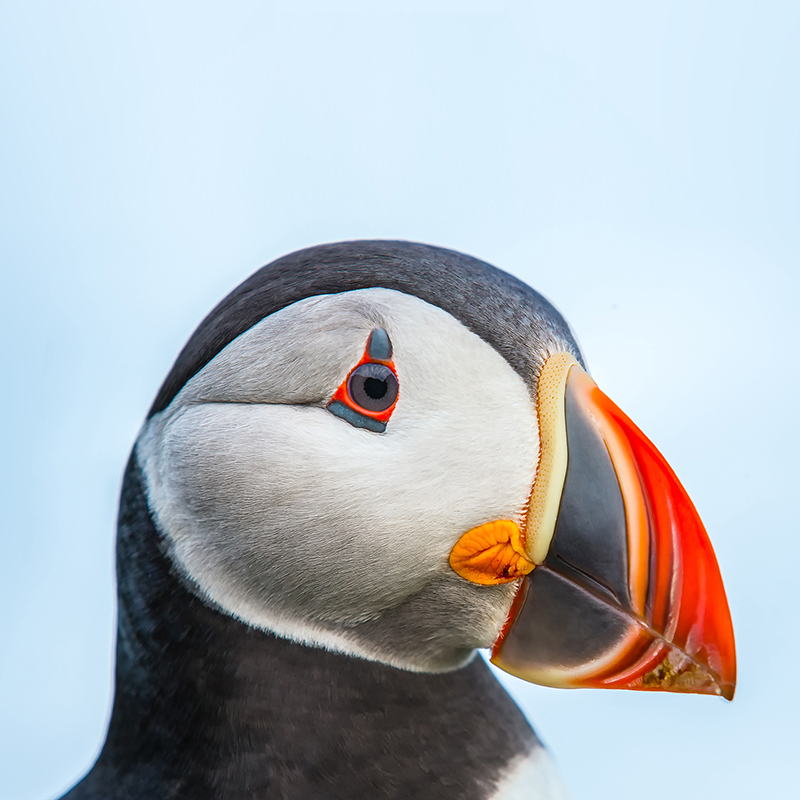
\includegraphics[width=\linewidth]{puffin}
            \caption{puffin Image}\label{fig:puffin7}
        \end{subfigure}
        \caption{A sample of multiple puffins}
        \label{fig:puffinall}
    \end{figure}
\end{Verbatim}
\begin{figure} [H]
    \centering
    \begin{subfigure}[b]{.45\linewidth}
        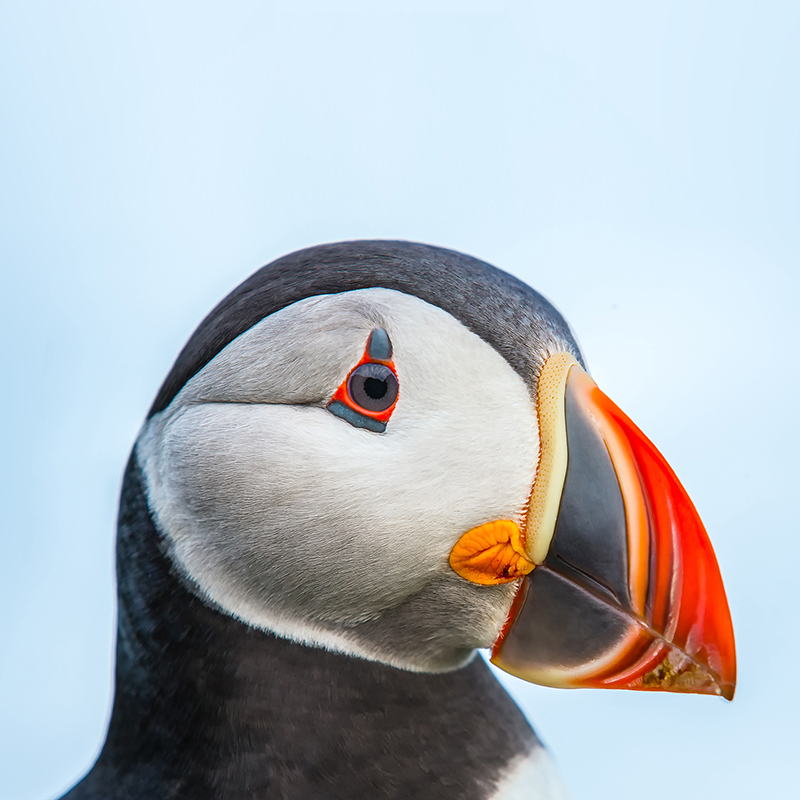
\includegraphics[width=\linewidth]{puffin}
        \caption{Useless Image}\label{fig:puffin1}
    \end{subfigure}
    \begin{subfigure}[b]{.45\linewidth}
        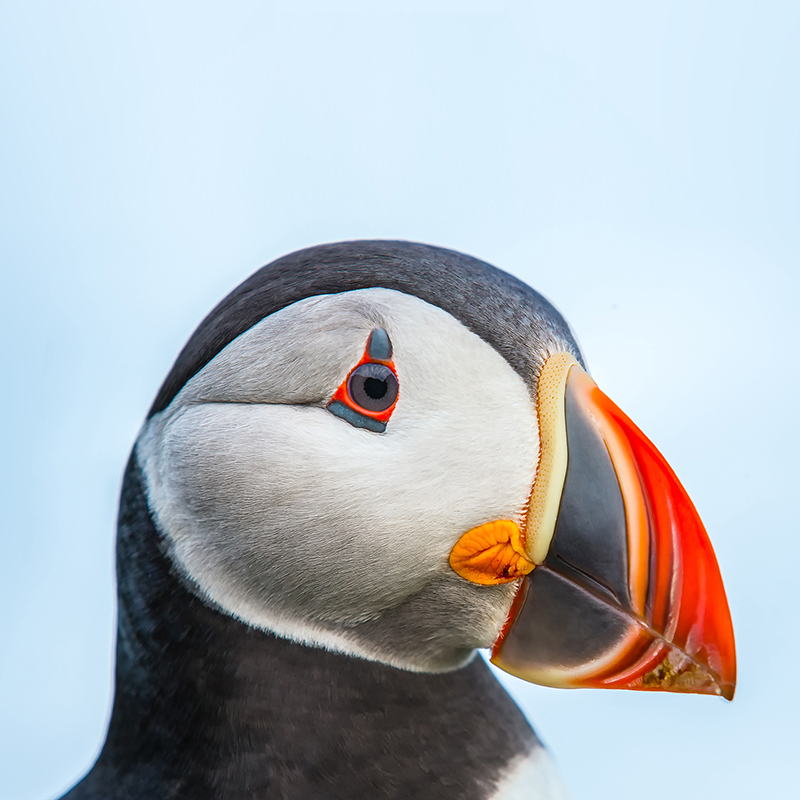
\includegraphics[width=\linewidth]{puffin}
        \caption{puffin Image}\label{fig:puffin2}
    \end{subfigure}

    \begin{subfigure}[b]{.45\linewidth}
        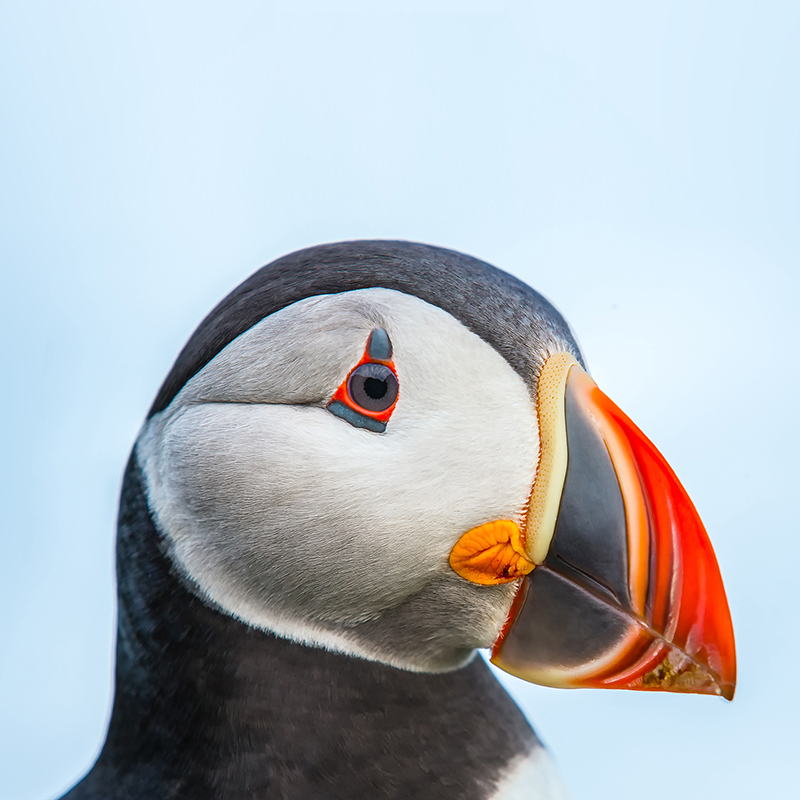
\includegraphics[width=\linewidth]{puffin}
        \caption{puffin Image}\label{fig:puffin4}
    \end{subfigure}
    \begin{subfigure}[b]{.45\linewidth}
        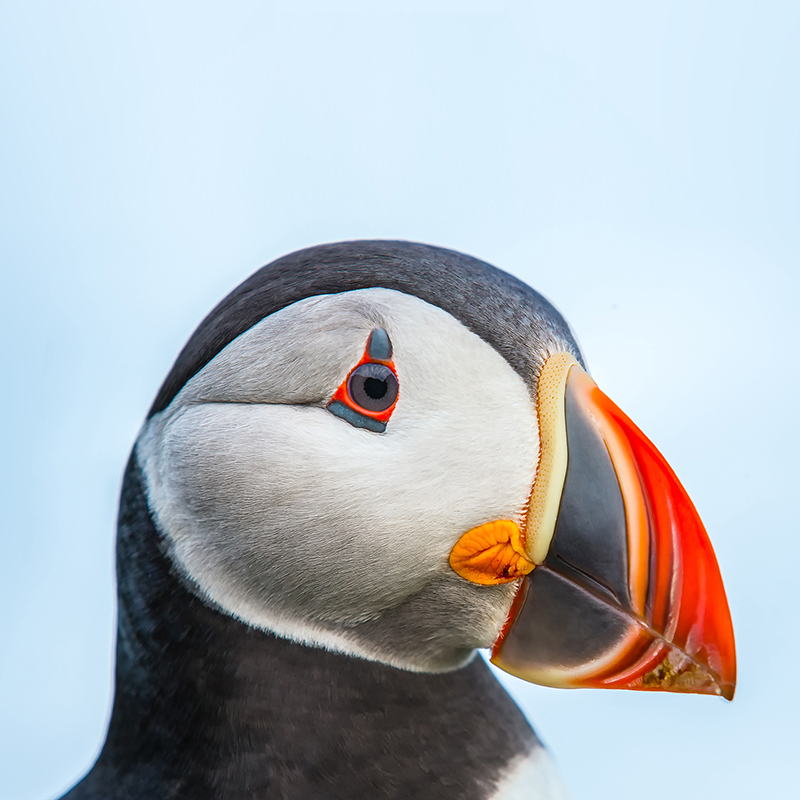
\includegraphics[width=\linewidth]{puffin}
        \caption{puffin Image}\label{fig:puffin5}
    \end{subfigure}

    \begin{subfigure}[b]{.45\linewidth}
        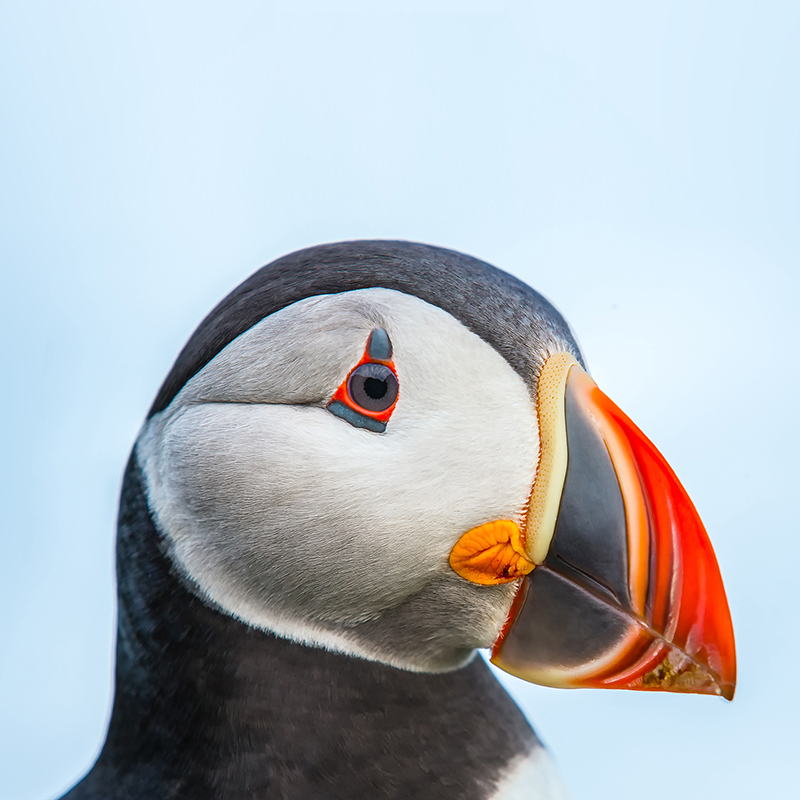
\includegraphics[width=\linewidth]{puffin}
        \caption{puffin Image}\label{fig:puffin6}
    \end{subfigure}
    \begin{subfigure}[b]{.45\linewidth}
        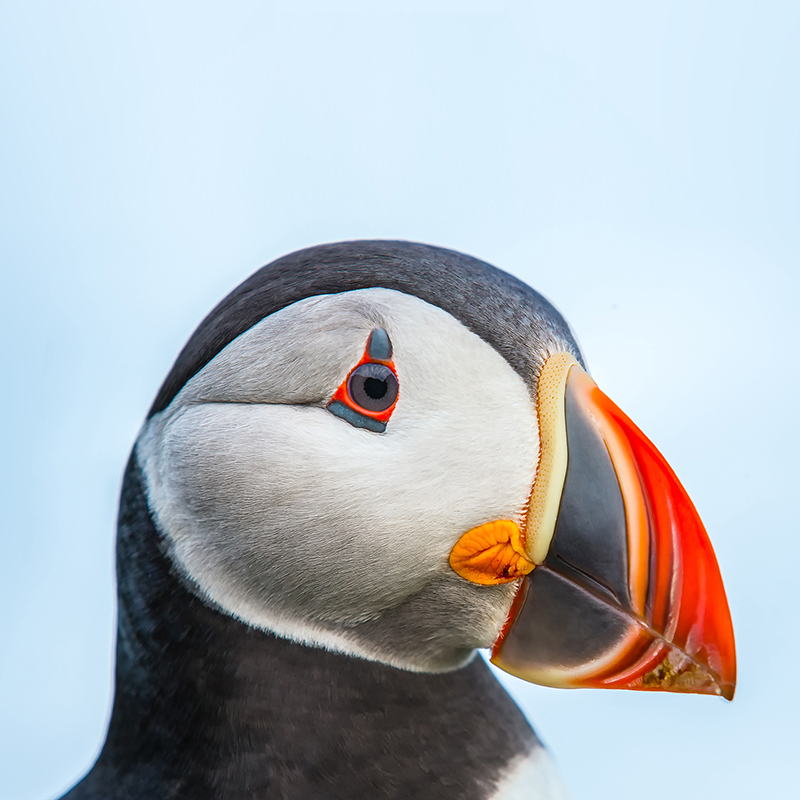
\includegraphics[width=\linewidth]{puffin}
        \caption{puffin Image}\label{fig:puffin7}
    \end{subfigure}
    \caption{A sample of multiple puffins}
    \label{fig:puffinall}
\end{figure}
\faWarning\, Notice here we used \verb=\subsection{Multiple images}= to create this subsection.
\subsection{Wrapped Images}
\begin{wrapfigure}{r}{0.35\textwidth}
    \centering
    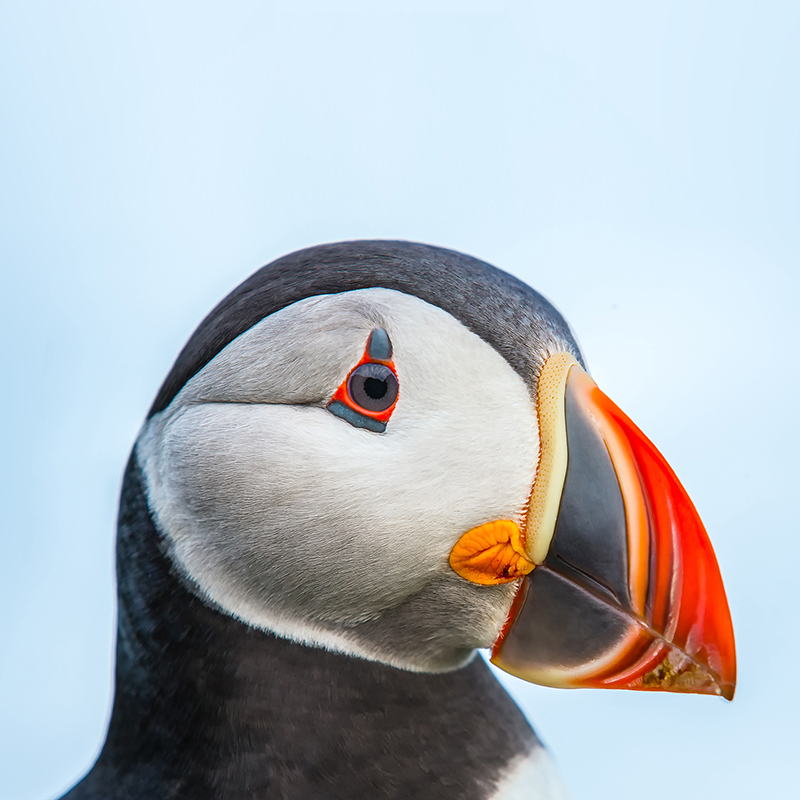
\includegraphics[width=0.3\textwidth]{puffin.jpg}
\end{wrapfigure}
You can place images next to text. For this we are using the \emph{wrapfig} package. I will add some random text here to see the effect.
\blindtext
\begin{Verbatim}[fontsize=\relsize{-1.5}]
    \begin{wrapfigure}{r}{0.35\textwidth}
        \centering
        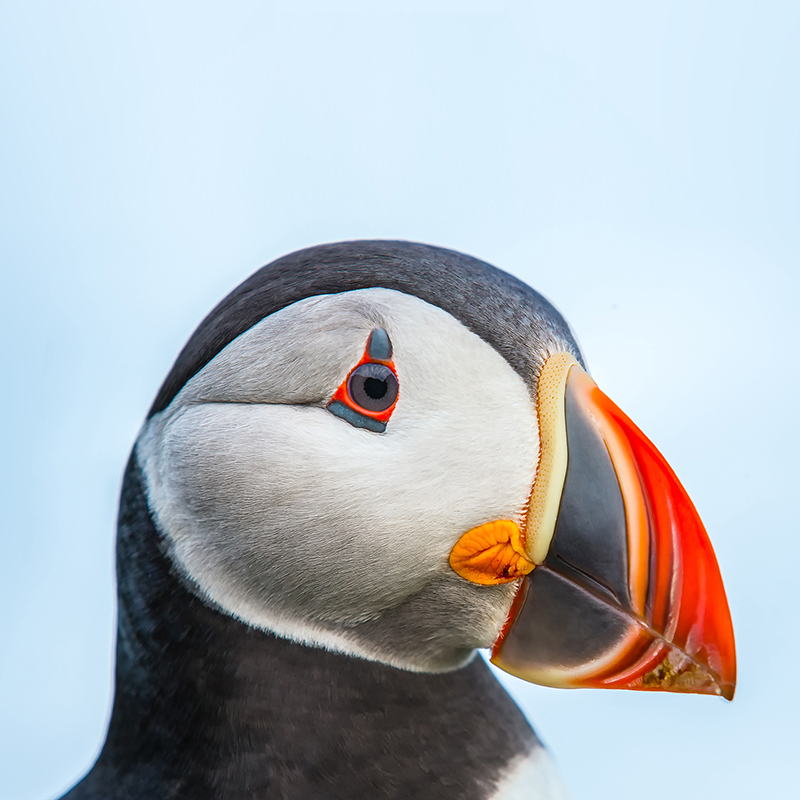
\includegraphics[width=0.3\textwidth]{puffin.jpg}
    \end{wrapfigure}
\end{Verbatim}
\section{Tables}
To start a table we use \verb=\begin{table}=. Check here for more \url{https://en.wikibooks.org/wiki/LaTeX/Tables}.

\faWarning\, \verb=[ht]= after \verb=\begin{table}[ht]= tells LaTeX that you prefer to place this "here" based on its order in the source LaTeX, or at the "top" of current page. Check this answer if you are interested in knowing more \url{https://tex.stackexchange.com/a/39020}.
\begin{Verbatim}[fontsize=\relsize{-1.5}]
    \begin{table}[ht]
        \caption{Sample of keywords in data set} % title of Table
        \centering % used for centering table
        \label{tab:numofimages}
        \begin{tabular}{c c c c c} % centered columns (4 columns)
            \hline % inserts single horizontal line
            Total  & Houses & Offices & Health-care & Hotels \\ [0.5ex] % inserts table
            \hline % inserts single horizontal line
            65,000 & 30,607 & 7,669   & 2,664       & 1,313  \\ [1ex] % [1ex] adds vertical space
            \hline
        \end{tabular}
    \end{table}
\end{Verbatim}
\begin{table}[ht]
    \caption{Sample of keywords in data set} % title of Table
    \centering % used for centering table
    \label{tab:numofimages}
    \begin{tabular}{c c c c c} % centered columns (4 columns)
        \hline % inserts single horizontal line
        Total  & Houses & Offices & Health-care & Hotels \\ [0.5ex] % inserts table
        \hline % inserts single horizontal line
        65,000 & 30,607 & 7,669   & 2,664       & 1,313  \\ [1ex] % [1ex] adds vertical space
        \hline
    \end{tabular}
\end{table}
%\pagebreak
\section{Source Code}
For source code we are using \emph{Minted}. To format the code correctly we are placing it inside \emph{minted} environment
\begin{verbatim}
    \begin{minted}[numbers=left,firstnumber=1,breaklines]{HTML}
        ...
    \end{minted}
    \end{verbatim}

\faWarning\, Formatting is set in \emph{MainPackages.tex} \verb=\usemintedstyle{tango}=. Check here for the rest of the styles and the supported languages \url{https://www.overleaf.com/learn/latex/Code_Highlighting_with_minted#Reference_guide}.

\begin{Verbatim}[fontsize=\relsize{-1.5}]
    \begin{listing}[h]
        \caption{Sample HTML code}
        \label{lis:html}
        \begin{minted}[numbers=left,firstnumber=1,breaklines]{HTML}
<!DOCTYPE html>
<html lang="en">
<head>
    <meta charset="UTF-8">
    <meta name="viewport" content="width=device-width, initial-scale=1.0">
    <title>Document</title>
</head>
<body>
</body>
</html>
    \end{minted}
    \end{listing}
\end{Verbatim}
\begin{listing}[h]
    \caption{Sample HTML code}
    \label{lis:html}
    \begin{minted}[numbers=left,firstnumber=1,breaklines]{HTML}
<!DOCTYPE html>
<html lang="en">
<head>
    <meta charset="UTF-8">
    <meta name="viewport" content="width=device-width, initial-scale=1.0">
    <title>Document</title>
</head>
<body>
</body>
</html>
    \end{minted}
\end{listing}
%\pagebreak
\section{Pseudo-Code}
For pseudo-code we are using \emph{Algorithm} and \emph{Algpseudocode} packages.
Using those packages when creating a pseudo-code you always need to indicate the end of a \emph{for} loop or an \emph{if} statement or a \emph{function}, imagine it as opening and closing your curly braces. Its a bit annoying though if they get rendered at the end, thats why when we loaded the package, we chose to activate an option called \emph{noend} \verb=\usepackage[noend]{algpseudocode}=, to stop those end of lines to be rendered.

Note the use of \verb=[1]= after \verb=\begin{algorithmic}[1]=, this activates the line numbers, remove it if you don't want the lines to be numbered.

\faWarning\, Note the use of \verb=[H]= after \verb=\begin{listing}[H]= this is from the \emph{Floating} package, it forces the figure/listing to appear exactly where we have it in the \emph{.tex} file, otherwise depending on it's size and to keep the flow of text consistent it might be moved up or down in the pages.

\faWarning\, In the \emph{Preamble} file we added
\begin{verbatim}
    renewcommand\listoflistingscaption{List of source codes}
    \listoflistings
\end{verbatim}
which allows us to create a table of listings, and call it \emph{Source code List}. That is why here we start with \verb=\begin{listing}= instead  of \verb=\begin{figure}=.

\faWarning\, Most of the function and variable names are wrapped in \verb=$...$=, this displays them differently, this is used to display inline formulas, but also gives text different styling, i.e. Normal Text vs $In Line Formula Text$.

Check here for more \url{https://en.wikibooks.org/wiki/LaTeX/Algorithms}, \url{http://tug.ctan.org/macros/latex/contrib/algorithmicx/algorithmicx.pdf}.

\begin{Verbatim}[fontsize=\relsize{-1.5}]
    \begin{listing}[H]
        \caption{Web Scrapper}
        \label{Algo:webscrapper}
        \begin{algorithmic}[1]
            \Function {$Spider$}{}
            \If {$startUrl$}
            \State $PARSE \gets startUrl$
            \EndIf
            \Function {$PARSE$}{}
            \State $parsed \gets url.response$
            \ForAll {$nextPages$ in $parsed.XPath(NextPageRule).extract$}
            \State $PARSE \gets nextPages$
            \EndFor
            \ForAll {$projectsUrl$ in $parsed.XPath(ProjectRule).extract$}
            \State $PROJECTPARSE \gets projectsUrl$
            \EndFor
            \EndFunction
            \Function {$PROJECTPARSE$}{}
            \State $parsed \gets url.response$
            \ForAll {$images$ in $parsed.XPath(ImageRules).extract$}
            \State $Export \gets \{imgUrl, imgName, projectId, projectTitle, keywords\}$
            \EndFor
            \EndFunction
            \EndFunction
        \end{algorithmic}
    \end{listing}
\end{Verbatim}
\begin{listing}[H]
    \caption{Web Scrapper}
    \label{Algo:webscrapper}
    \begin{algorithmic}[1]
        \Function {$Spider$}{}
        \If {$startUrl$}
        \State $PARSE \gets startUrl$
        \EndIf
        \Function {$PARSE$}{}
        \State $parsed \gets url.response$
        \ForAll {$nextPages$ in $parsed.XPath(NextPageRule).extract$}
        \State $PARSE \gets nextPages$
        \EndFor
        \ForAll {$projectsUrl$ in $parsed.XPath(ProjectRule).extract$}
        \State $PROJECTPARSE \gets projectsUrl$
        \EndFor
        \EndFunction
        \Function {$PROJECTPARSE$}{}
        \State $parsed \gets url.response$
        \ForAll {$images$ in $parsed.XPath(ImageRules).extract$}
        \State $Export \gets \{imgUrl, imgName, projectId, projectTitle, keywords\}$
        \EndFor
        \EndFunction
        \EndFunction
    \end{algorithmic}
\end{listing}

%\pagebreak
\section{Text}
Some things you can use to style your text,
\begin{itemize}
    \item Writing function names, use \verb=\textproc{ThisIsAFunctionName}= \textproc{ThisIsAFunctionName}.
    \item Emphasize a word using \verb=\emph{emphasized text}= \emph{emphasized text}.
    \item Make text bold using \verb=\textbf{this text is bold}= \textbf{this text is bold}.
    \item Underline text using \verb=\underline{this is underlined}= \underline{this is underlined}.
\end{itemize}